\section{Simulationen}

Um den Einfluss von CAPE auf den Aufwind und die Produktion von Hagel in einer Superzelle zu untersuchen, wird das \textit{Cloud Model 1} (CM1), Version 20.2, \parencite{bryan2002} verwendet. Die Simulationen werden auf einem stationären Gitter der Auflösung \(\num{480}\times\num{360}\times\num{80}\) durchgeführt, dabei wird ein horizontaler Gitterpunktabstand von \SI{500}{\m} und ein vertikaler von \SI{250}{\m} gewählt. Folglich führt dies zu einem Simulationsraum von \(\SI{240}{\km}\times\SI{180}{\km}\times\SI{20}{\km}\). Der Zeitschritt beträgt \SI{1.5}{\s} und die Gesamtdauer der Simulation ist \SI{3}{\hour}, dabei werden Zwischenergebnisse alle \SI{5}{\min} abgespeichert.

\begin{table}
	\centering
	\begin{tabular}{ccS[table-format=4.1]}
		\toprule
		Label & Mischungsverhältnis [\si{\g\per\kg}] & {CAPE [\si{\J\per\kg}]} \\
		\midrule
		\texttt{MR11} & 11 & 533.5  \\
		\texttt{MR14} & 14 & 1857.7 \\
		\texttt{MR16} & 16 & 2984.9 \\
		\texttt{MR21} & 21 & 5912.5 \\
		\bottomrule
	\end{tabular}
	\caption{Durchgeführte CM1-Simulationen}
	\label{tab:sims}
\end{table}

\begin{figure}
	\centering
	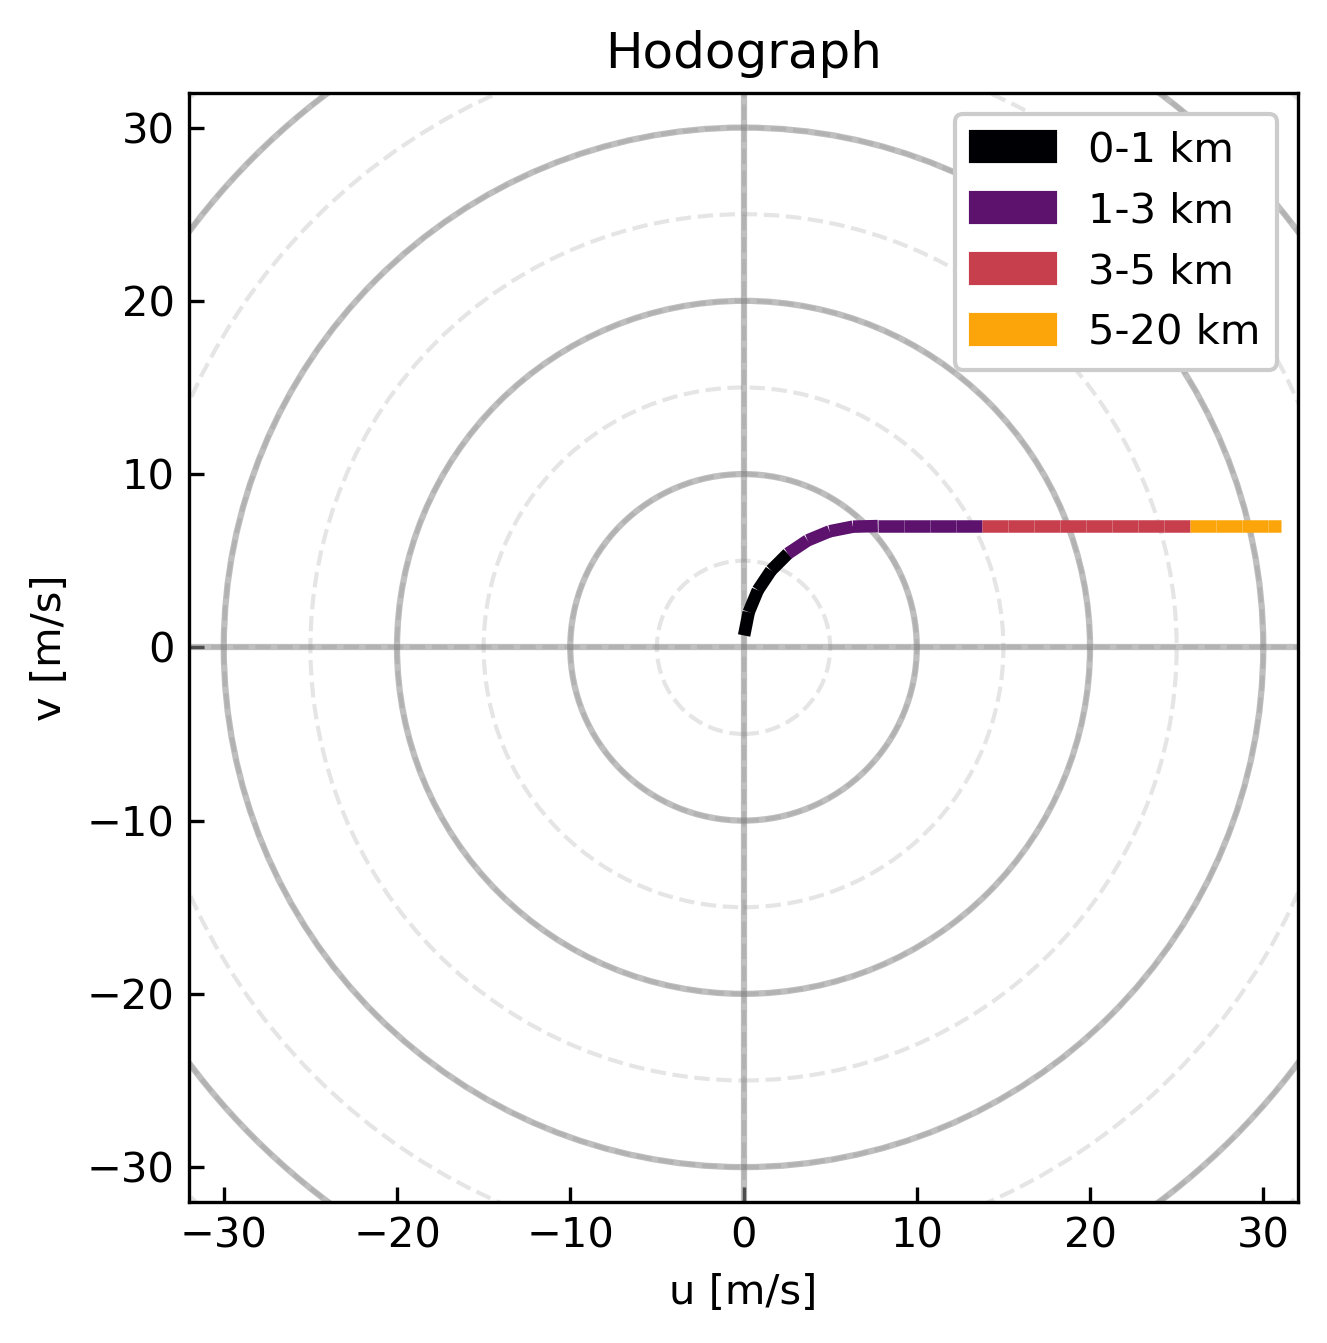
\includegraphics[width=0.6\linewidth]{../figs/hodograph.png}
	\caption{Der Hodograph zeigt die Veränderung des Windprofils mit der Höhe. Das idealisierte \textit{quarter-circle} Windprofil \parencite{weisman2000} wird in allen Simulationen unverändert verwendet.}
	\label{fig:hodograph}
\end{figure}

Die Konvektion wird durch eine Wärmeblase mit einem Temperaturunterschied von \SI{2}{\K} ausgelöst. Diese besitzt eine horizontale Ausprägung von \SI{20}{\km}, ist \SI{3}{\km} hoch und befindet sich im südwestlichen Bereich der Domain. Die Mikrophysik wird durch das \textit{two-moment Morrison scheme} \parencite{morrison2005} parametrisiert. Das Windprofil ist ein idealisierter \textit{quarter-circle} nach \textcite{weisman2000} und in \cref{fig:hodograph} dargestellt. Die Soundings der Simulationen basieren auf \textcite{weisman1982} und führen typischerweise zur Bildung von Superzellen. In den Soundings wird nun das Mischungsverhältnis von Wasserdampf zu trockener Luft erhöht (vgl. \cref{tab:sims}), was durch das niedrigere Einsetzen der Feuchtekonvektion das CAPE der Atmosphäre zu Beginn der Simulation verändert. Die gewählten Werte sind dabei aus \textcite{weisman1982} übernommen, allerdings stellt der maximale Wert des Mischungsverhältnisses \(q_v = \SI{21}{\g\per\kg}\) eine Situation dar, in der Feuchtekonvektion bereits direkt am Boden einsetzt. \(q_v\) wird dabei derart gewählt, dass bei gegebenem Umgebungsdruck und -temperatur die relative Luftfeuchtigkeit \SI{100}{\percent} beträgt. Die entsprechenden Profile sind in \cref{fig:sounding} dargestellt.

\begin{figure}
	\centering
	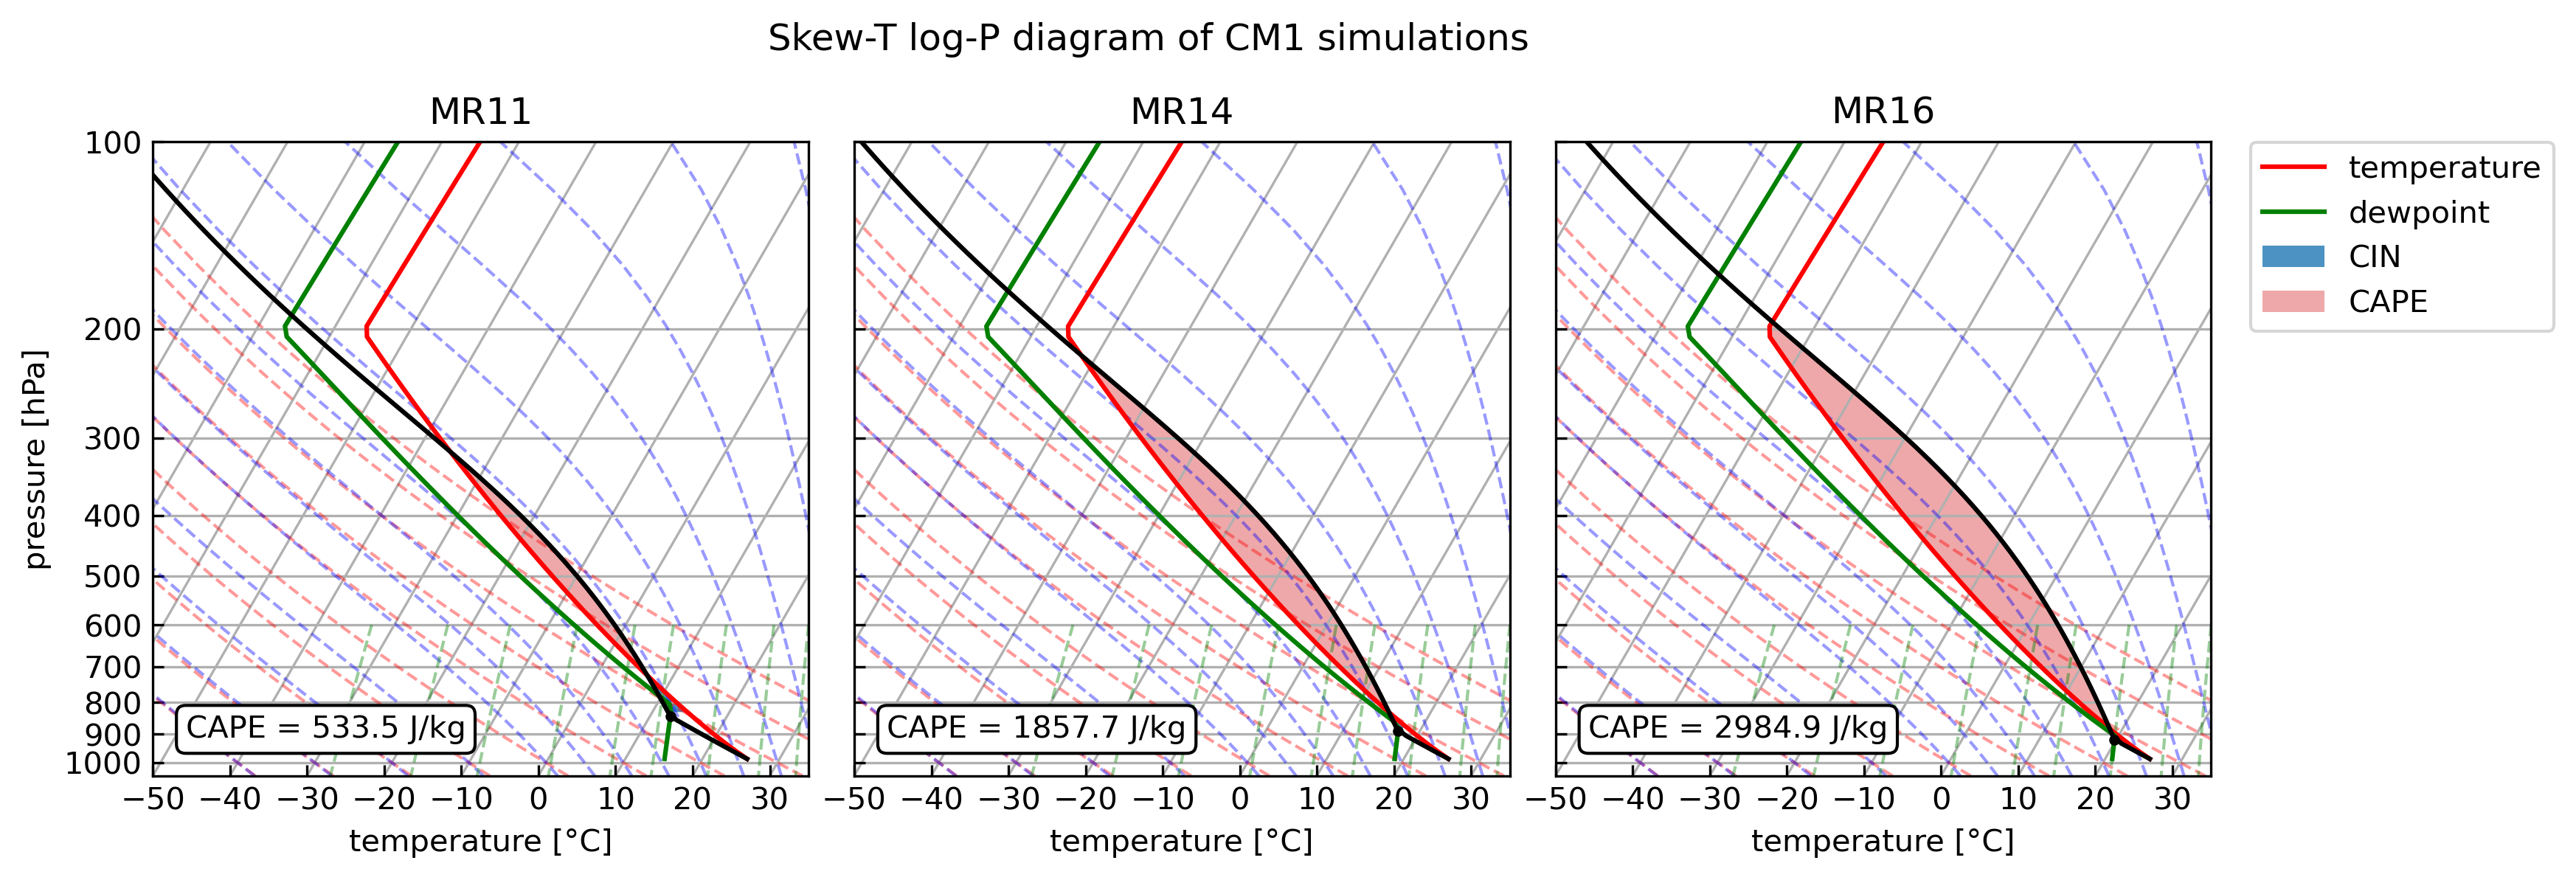
\includegraphics[width=\linewidth]{../figs/sounding.png}
	\caption{Die Soundings der einzelnen CM1-Simulationen mit vertikalem Temperatur- und Taupunktprofil. Außerdem stellt die schwarze Kurve den Aufstieg eines Luftpakets dar -- zunächst trockenadiabatisch bis zum markierten Punkt, dann setzt Feuchtekonvektion ein. Aus der Fläche zwischen Umgebungstemperatur und Temperatur des Luftpakets kann das CAPE bestimmt werden. \textit{Skew-T} betont die geneigten Isothermen.}
	\label{fig:sounding}
\end{figure}
